\documentclass[border=5pt]{standalone}
\usepackage{tikz}
\usepackage{amsmath}
\usetikzlibrary{calc,intersections}
\usepackage{pgfplots}
\pgfplotsset{compat=1.16}
\usepgfplotslibrary{polar}
\begin{document}
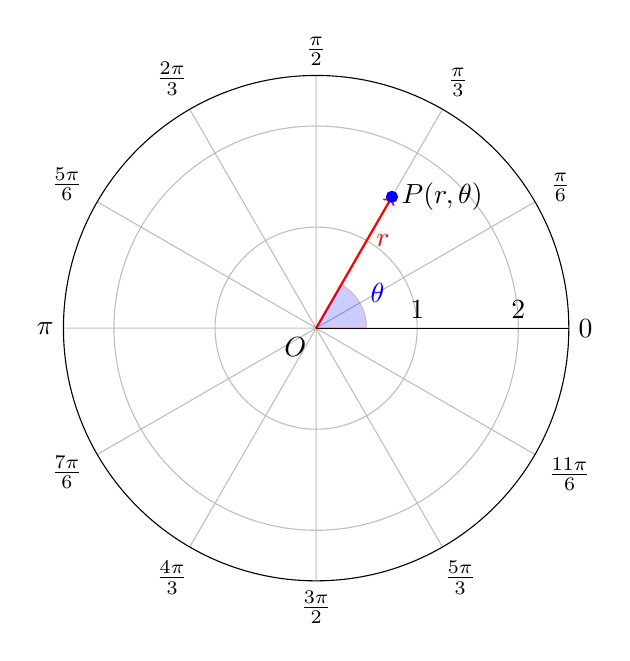
\begin{tikzpicture}
\begin{polaraxis}[
    width=8cm,
    height=8cm,
    grid=both,
    xticklabel=$\theta=\pgfmathprintnumber{\tick}$,
    yticklabel=$r=\pgfmathprintnumber{\tick}$,
    xmin=0, xmax=360,
    ymin=0, ymax=2.5,
    xtick={0,30,...,330},
    ytick={1,2},
    xticklabels={$0$,$\frac{\pi}{6}$,$\frac{\pi}{3}$,$\frac{\pi}{2}$,$\frac{2\pi}{3}$,$\frac{5\pi}{6}$,$\pi$,$\frac{7\pi}{6}$,$\frac{4\pi}{3}$,$\frac{3\pi}{2}$,$\frac{5\pi}{3}$,$\frac{11\pi}{6}$},
    yticklabels={1,2},
    tick style={draw=none}
]
    % Sample point
    \addplot[only marks, mark=*, blue, mark size=2pt] coordinates {(60,1.5)};
    \node[right] at (axis cs:60,1.5) {$P(r,\theta)$};

    % Highlight r and theta
    \draw[red, thick, ->] (axis cs:0,0) -- (axis cs:60,1.5);

    \pgfplotsset{cycle list={{}}}
    \addplot[red, fill=blue, opacity=0.2, domain=0:60, samples=100]
        {0.5} -- (axis cs:0,0) -- cycle;

    % Labels
    \node[red, right] at (axis cs:60,1) {$r$};
    \node[blue] at (axis cs:30,0.7) {$\theta$};

    % Origin
    \node[below left] at (axis cs:0,0) {$O$};
\end{polaraxis}
\end{tikzpicture}
\end{document}
